\section{Tecnologías utilizadas}

\subsection{Sistema de recomendación}
El RS de R.Sánchez y col. utiliza LightFM\footnote{LightFM es una implementación en python de varios algoritmos populares de recomendación.} para crear los modelos de IA. Para implementar el FL se ha tenido que modificar gran parte del RS previo y se ha tenido que hacer uso de las utilidades que proporciona LightFM que se van a explicar en los siguientes apartados. 
\subsubsection{Creación del modelo}
El paso de creación del modelo es un paso complejo puesto que conlleva la correcta gestión de muchos datos e información. Asimismo, estos datos han de estar correctamente estructurados y construidos, puesto que LightFM requiere que la información este convertida a matrices dispersas y no tolera elementos vacíos en ellas. Para ello LightFM provee de herramientas de creación de datasets que facilitan la creación de las matrices, de forma que sea más fácil incluirlas en el modelo. 
\\ \\
Entre estas herramientas se encuentran:

\begin{itemize}
    \item \textit{build\_user\_features($\ldots$)} \quad Permite crear la matriz CSR de usuarios y atributos de usuarios.
    \item \textit{build\_item\_features($\ldots$)} \quad Permite crear la matriz CSR  de items y atributos de items.
    \item \textit{build\_interactions($\ldots$)} \quad Permite crear las matriz COO de interacciones y las matriz COO de sus correspondientes pesos.
\end{itemize}

Hay que tener en cuenta que las matrices CSR (Compressed Sparse Row) hacen referencia a las matrices que admiten operaciones matriciales y acceso eficientemente; y que las matrices COO (Coordinate list) hacen referencia a las matrices que soportan modificaciones eficientemente, son generalmente utilizadas para construir matrices.


\paragraph{Atributos de los usuario}
Para crear el modelo, es necesario entre otras cosas, disponer de las características de los usuarios. En este caso contamos con multitud de atributos sobre cada usuario (véase la tabla \ref{tab:AtributosUsuarios}).
\\ \\
Para convertir toda esa información del usuario a la matriz CSR que exige LightFM habrá que llamar a \textit{build\_user\_features($\ldots$)} con los IDs de usuario y sus atributos, formando una lista que tenga listas de los IDs de los usuarios con sus listas de atributos, es decir:

\begin{figure}[H]
    \centering
    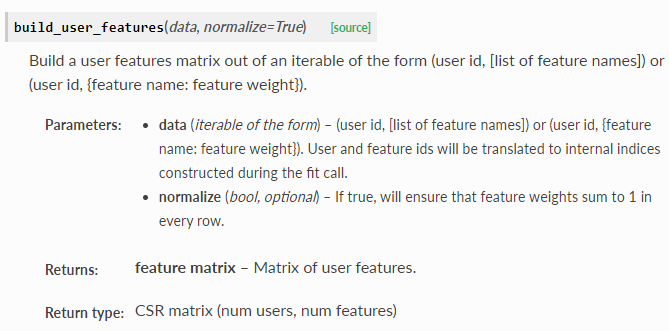
\includegraphics[width=0.9\textwidth]{Figuras/LightFM_build_user_features.png}    
    \caption{Creación de la matriz de atributos de usuario} 
    \label{fig:BuildUserFeatures}
\end{figure}

\paragraph{Atributos de los elementos}
Además de los usuarios y de sus atributos, también se ha de disponer de los elementos a ordenar en el ranking, llamados items, y de sus características. En este caso estos items representan las estrategias de persuasión por las que se preguntó a los usuarios en el cuestionario. Sin embargo, al contrario que en el punto anterior, no contamos con tantos atributos sobre estos items, sino que cada estrategia de persuasión cuenta con dos atributos llamados dimensiones. Estos atributos no se encuentran presente en todas las estrategias, lo que da como resultado que haya algunas que tengan dos, una o ninguna dimension (véase la tabla \ref{tab:EstrategiasPersuasion}).
\\ \\
Para convertir toda esa información de los items a la matriz CSR que exige LightFM habrá que llamar a \textit{build\_item\_features($\ldots$)} con los IDs de las estrategias y y sus atributos, formando una lista que tenga listas de los IDs de las estrategias con sus listas de atributos, es decir:

\begin{figure}[H]
    \centering
    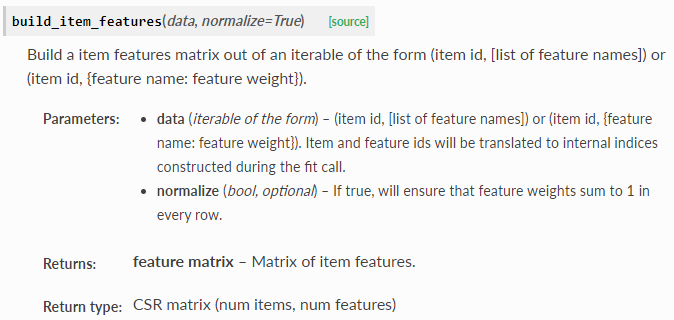
\includegraphics[width=0.9\textwidth]{Figuras/LightFM_build_item_features.png}    
    \caption{Creación de la matriz de atributos de los elementos} 
    \label{fig:BuildItemFeatures}
\end{figure}

\paragraph{Interacciones}
Para crear las interacciones de entrenamiento y de testeo LightFM nos facilita un método para poder crearlo fácilmente. Esta herramienta se utilizará dos veces como mínimo, una con los identificadores y atributos de los usuarios que serán utilizados para entrenar el modelo y la otra para generar las interacciones de los usuarios con los que se quiere realizar las predicciones.
\begin{figure}[H]
    \centering
    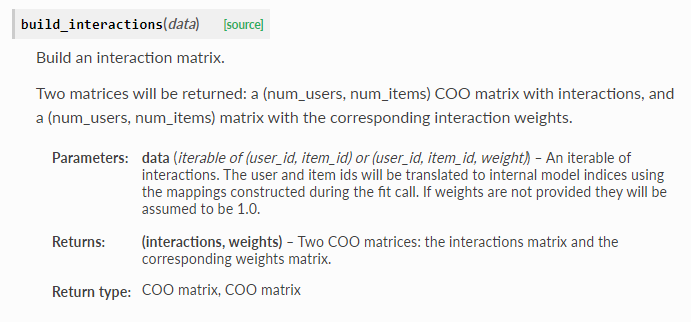
\includegraphics[width=0.9\textwidth]{Figuras/LightFM_build_interactions.png}    
    \caption{Creación de la matriz de interacciones} 
    \label{fig:BuildInteractions}
\end{figure}

\subsubsection{Ajuste}
Para permitir que el modelo pueda ser reajustado con nuevos datos y permitir el aprendizaje incremental LightFM implementa una variante de la herramienta \textit{fit($\cdots$)}. En un principio \textit{fit($\cdots$)} ajusta el modelo pero si se vuelve a utilizar esta herramienta se reajusta desde cero, sin mantener ningún dato insertado en el modelo antes.
\\ \\
Para solucionar esto LightFM tiene una variante llamada \textit{fit$\_$partial($\cdots$)}, esta herramienta permite ajustar datos al modelo tantas veces como se quiera sin perder los datos insertados previamente.
\begin{figure}[H]
    \centering
    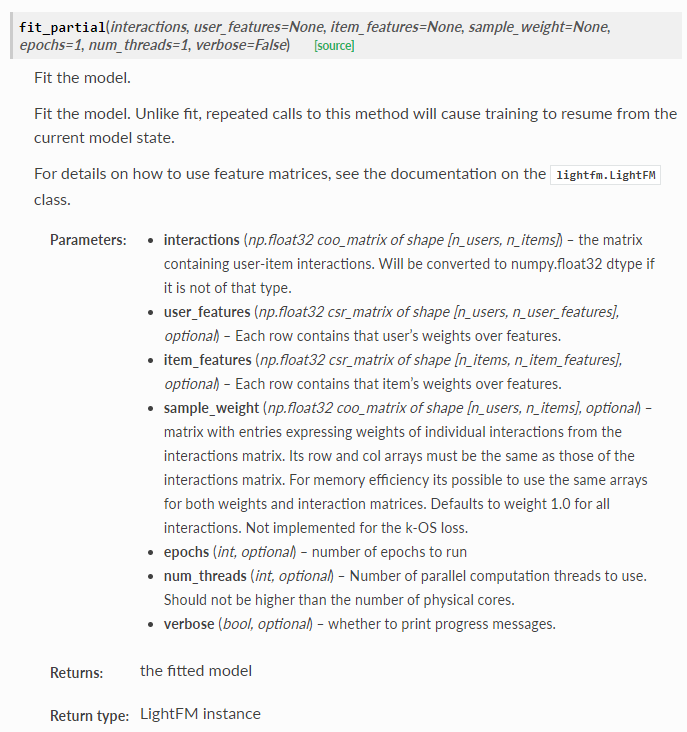
\includegraphics[width=0.9\textwidth]{Figuras/LightFM_fit_partial.png}    
    \caption{Ajustar datos al modelo} 
    \label{fig:FitPartial}
\end{figure}

\subsubsection{Predicción}
Para generar las predicciones LightFM implementa un método que sintetiza el proceso y permite que insertando los interacciones de test se prediga el ranking para estos usuarios.
\begin{figure}[H]
    \centering
    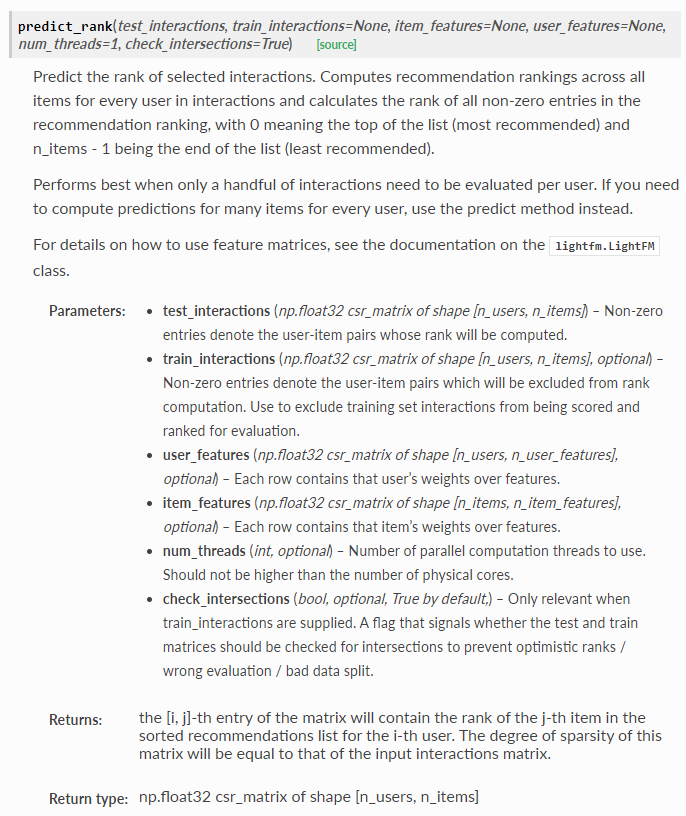
\includegraphics[width=0.9\textwidth]{Figuras/LightFM_predict_rank.png}    
    \caption{Ajustar datos al modelo} 
    \label{fig:FitPartial}
\end{figure}
\subsubsection{Evaluación}
La evaluación de los resultados obtenidos de las predicciones de los modelos es un apartado fundamental que permite analizar la eficacia de estas predicciones. Además, la utilización de métricas y técnicas permitirá poder comparar los resultados entre sí para poder demostrar si la predicción es correcta, aceptable o errónea.
\\ \\
Para este caso no se incluirá ninguna métrica ni método de LightFM, sino que se utilizará la métrica NDPM implementada y explicada en el apartado de valoración \ref{Valoracion}.


\subsection{Memoria}
La memoria técnica de este proyecto ha sido elaborada en \LaTeX. Esta ha sido escrita en el editor de código \textit{Visual Studio Code} gracias al complemento \textit{LaTeX Workshop}, que proporciona las características básicas para la composición tipográfica de \LaTeX $ $ en \textit{Visual Studio Code}, y gracias a \textit{MiKTeX}, distribución Tex para Windows, la cual permite la compilación de documentos \LaTeX $ $ en Windows.
\\ \\
Además, para controlar el avance y las versiones de la memoria se ha utilizado el controlador de versiones GIT. Para que las versiones no permaneciesen en el ordenador local se decidió abrir un repositorio en GitHub\footnote{Repositorio: $https://github.com/Ibaii99/PFG\_MEMORIA$} donde se ha ido desarrollando este proyecto.
\\ \\
Para la gestión bibliográfica se ha utilizado \textit{Zotero}, herramienta que permite gestionar las citas bibliográficas a través de una app y un complemento en el navegador. Para exportar estas referencias a \LaTeX $ $ se ha utilizado el paquete \textit{BibTex}.
\subsection{Desarrollo}
El desarrollo de este proyecto se ha realizado en el editor \textit{Visual Studio Code} y con el leguaje de programación \textit{Python}, al igual que la memoria se ha utilizado el controlador de versiones GIT con un repositorio en Github. A lo largo del desarrollo del proyecto han surgido diferentes necesidades que se han ido solucionando con la incorporación de ciertas herramientas, estas herramientas han sido agrupadas en función de las necesidades que han solventado en el proyecto, se detallan a continuación.
\subsubsection{Matrices}
A la hora de gestionar matrices de grandes dimensiones se ha utilizado la biblioteca \textit{NumPy}, la cual da soporte para crear grandes matrices multidimensionales y realizar operaciones matemáticas de alto nivel con ellas. 
\\ \\
Se han usado matrices NumPy tanto para la gestión de la información y estructurar los datos en LightFM como para realizar las tareas del modelo de consenso.
\subsubsection{Cálculos estadísticos} 
A la hora de realizar los cálculos sobre las matrices de predicción en el modelo de consenso la mediana y moda han tenido que ser aplicadas con distintas librerías. Aunque se ha intentado utilizar \textit{NumPy} para todo esta biblioteca no contaba con ningún método que permitiera calcular la moda de una lista, por lo cual ha habido que importar una biblioteca extra, \textit{SciPy}.
\\ \\
\textit{SciPy} permite aplicar bastantes algorítmos y herramientas matemáticas, pero solo se ha importado su paquete de funciones estádisticas \textit{stats}. 
\subsubsection{Guardado de los modelos}
Uno de los principales problemas del proyecto era el envío de los modelos y para ello se necesitaba exportar el modelo a un fichero para poder enviarlo por la red. Como LightFM permite la serialización de sus modelos se elijió la biblioteca \textit{pickle} para este proceso. Esta biblioteca implementa módulos binarios para la serialización y deserialización, por lo cual permitia tanto guardar a fichero el modelo como importarlo desde un fichero.
\subsubsection{Securización} 
Para la implementación de la seguridad en las comunicaciones y realizar las operaciones criptográficas se ha utilizado el paquete \textit{cryptography}, este paquete provee de métodos de cifrado y descifrado simétricos y asimétricos de alto nivel, lo que permite un nivel de abstracción mayor y por ende una más fácil gestión. 
\subsubsection{Compresión}
Un elemento fundamental del proyecto era minimizar el volumen de las comunicaciones puesto que es uno de los grandes inconvenientes del FL. Con el objetivo de minimizar el tamaño de las comunicaciones se identificaron donde se daban los mayores volúmenes de conexión y se averiguó que era en el intercambio de modelos entre los participantes y el servidor y viceversa. Para ello la compresión de las comunicaciones se realizó mediante la biblioteca \textit{zlib}. 
\subsubsection{Gestión de la ejecución}
Como en este proyecto se gestionan muchos dispositivos y se tiene que reproducir en protocolo de FL en orden es crucial poder controlar lo que se ejecuta en cada dispositivo. Para poder gestionarlo con más facilidad se ha implementado el paquete \textit{OptionParser} para poder definir ciertos \textit{flags} para especificar qué proceso se quiere ejecutar en el dispositivo.
\\ \\
En cuanto a los flags generales se encuentran:
\begin{itemize}
    \item \textit{-k}, para generar las claves públicas y privadas de encriptación.
    \item \textit{-e}, para encriptar los modelos con la clave pública del receptor.
    \item \textit{-d}, para desencriptar el modelo recibido con la clave privada propia.
\end{itemize}   
Sin embargo, debido al funcionamiento dispar del nodo respecto a los participantes hay diferentes \textit{flags} dependiendo del dispositivo, de esta forma las Raspberries cuentan con:
\begin{itemize}
    \item \textit{-t}, para generar un modelo LightFM y entrenarlo con los datos del país.
    \item \textit{-c}, para comparar el modelo reentrenado recibido con el que tiene el dispositivo.
    \item \textit{-v}, para realizar el entrenado del modelo y la encriptación.
    \item \textit{-w}, para desencriptar el modelo reentrenado y compararlo con el local.
    \item \textit{-a}, flag extra solo usado en desarrollo que permite simular virtualmente a los participantes, su única utilidad ha sido durante el desarrollo y no durante el RS.
\end{itemize}
A su vez, el nodo de agregación ha tenido también sus diferentes tareas:
\begin{itemize}
    \item \textit{-s}, para generar los datos sintéticos.
    \item \textit{-c}, consensuar los datos sintéticos con los modelos de los participantes.
    \item \textit{-v}, desencriptar el modelo del participante, generar los datos sintéticos, realizar el consenso de los datos y encriptar los modelos reentrenados.
\end{itemize}
\begin{figure}[H]
    \centering
    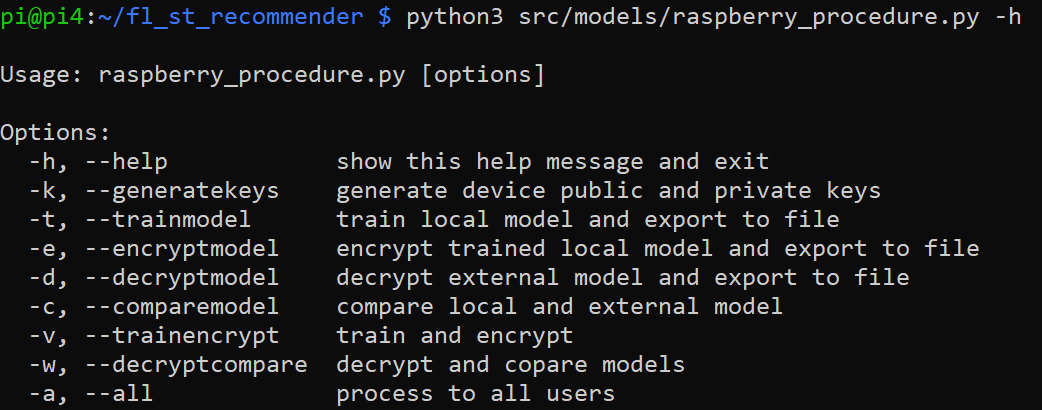
\includegraphics[width=0.8\textwidth]{Figuras/Raspberry_procedure_h.png}
    \caption{Opciones de ejecución de las Raspberries} 

    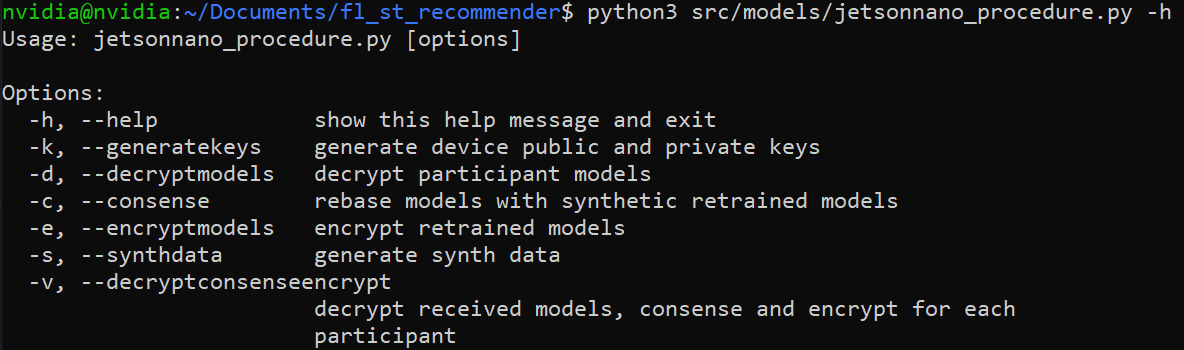
\includegraphics[width=0.8\textwidth]{Figuras/jetsonnano_procedure_h.png}
    \caption{Opciones de ejecución de la Jetson Nano} 
\end{figure}


\subsubsection{Aprovisionamiento}
Uno de los riesgos del proyecto que se ha incluido en la sección de gestión de riesgos ha sido la creación de un \textit{script} que permita automatizar la instalación de todos los paquetes necesarios para la ejecución del proyecto en caso de que una tarjeta SD se averiase.
\\ \\
Los \textit{script}s que se han desarrollado para cumplir con este objetivo han sido dos, uno de aprovisionamiento del sistema linux y otro de requisitos de paquetes python. En un proyecto normal hubiera valido con un simple script de requisitos de python \textit{requirements.txt} el cual alberga el nombre de los paquetes y la versión a instalar, proceso fácilmente realizable mediante el comando \textit{pip install -r requirements.txt}. Sin embargo, en este proyecto los paquetes que se utilizan no son fácilmente importables de un sistema operativo a otro, por lo que ha habido que desarrollar un pequeño script de aprovisionamiento en \textit{bash} que mediante consola instalase todos los paquetes necesario para el correcto funcionamiento de los paquetes python en las Raspberries y la Jetson Nano.
\\ \\
Cada tipo de dispositivo ha tenido su propio conjunto de ficheros de aprovisionamiento, de forma que ha habido un \textit{requirements.txt} y un script en \textit{bash} para las Raspberries y otro para la Jetson nano, ya que por sistema operativo, arquitectura y compatibilidades los dispositivos deben funcionar con distintas versiones de ciertos paquetes y en caso de las Raspberries con algún paquete más.

\subsubsection{Reporte de resultados}
Con el objetivo de representar los resultados de la precisión de los rankings de una forma vistosa y fácilmente entendible se incorporó la biblioteca \textit{Matplotlib} para la generación de gráficos. Esta biblioteca permite crear diversidad de gráficos para representar la información, elemento imprescindible a la hora de comparar el rendimiento del sistema.

\subsection{Sistemas operativos}
En cuanto a sistemas operativos se ha trabajado tanto con \textit{Windows} a la hora de realizar el desarrollo como con \textit{Linux} a la hora de realizar la implementación. Los sistemas \textit{Linux} que se han utilizado han sido \textit{RaspbianOS}, sistema operativo derivado de \textit{Debian} para las Raspberries con soporte oficial, y una adaptación de \textit{Ubuntu} para la Jetson Nano.
\subsection{Comunicaciones}
Como bien se ha explicado en el apartado de securización de las comunicaciones \ref{SegCom} para comunicarse con los dispositivos y poder parametrizarlos y configurar la instalación se utilizará el protocolo \textit{SSH}, el cual permite abrir una línea de comando desde un dispositivo a otro.
\\ \\
Además, para el intercambio de ficheros se ha utilizado el protocolo \textit{SCP}, el cual se apoya en gran parte del protocolo \textit{SSH} y al igual que este está explicado en el apartado de securización de las comunicaciones \ref{SegCom}.